\documentclass{beamer}

\usepackage{préambule}
\usepackage{amsmath,enumerate}

\setbeamersize{
	text margin left=0.5cm,
	text margin right=0.5cm
}

\newcounter{questionDepth}
\newcounter{questionCounteri}
\newcounter{questionCounterii}
\setcounter{questionDepth}{0}

\newcommand{\myItem}{\ifthenelse{\equal{\value{questionDepth}}{1}}{
	{\ifthenelse{\equal{\value{questionCounteri}}{0}}{}{\leavevmode\newline}\color{blue}\stepcounter{questionCounteri}\arabic{questionCounteri}.\space}
}{\ifthenelse{\equal{\value{questionDepth}}{2}}{
	{\ifthenelse{\equal{\value{questionCounterii}}{0}}{}{\leavevmode\newline}\color{blue}\stepcounter{questionCounterii}\phantom{\arabic{questionCounteri}.}\alph{questionCounterii}.\space}
}{}}}

\renewenvironment{question}{
\ifthenelse{\equal{\value{questionDepth}}{0}}{
	\stepcounter{questionDepth}
	\setcounter{questionCounteri}{0}
}{
	\stepcounter{questionDepth}
	\setcounter{questionCounterii}{0}
}
}{
\addtocounter{questionDepth}{-1}
}

\begin{document}

\small

\begin{frame}
	\setlength{\columnseprule}{0.7pt}
	\begin{multicols}{2}
		\begin{question}
			\myItem Une fonction $f$ est représentée sur le graphe suivant :
			\begin{center}
				\begin{tikzpicture}[scale=0.4]
					\draw[thin,gray] (-4.5,-1.5) grid (5.5,4.5);
					\draw[\myArrow] (-4.5,0) -- (5.5,0);
					\draw[\myArrow] (0,-1.5) -- (0,4.5);
					\draw[thick] (1,0) -- ++(0,-0.5) node[below] {$1$};
					\draw[thick] (0,1) -- ++(-0.5,0) node[left] {$1$};

					\draw[ultra thick,orange] (-4,-1) -- (-1,2) -- (1,0) -- (9/4,15/4) -- (5,1) node[above] {$𝒞_f$};
				\end{tikzpicture}
			\end{center}
			Déterminer :

			\begin{question}
				\myItem L'image de $1$, $3$ et $-1$
				\myItem Les antécédents de $3$, $0$ et $-0,5$
			\end{question}
			\myItem Soit $g$ la fonction telle que $g(x) = 0,5x - 3$. Déterminer :

			\begin{question}
				\myItem Les images de $3$, $6$ et $-1$
				\myItem Les antécédents de $-1$, $-9$ et $7$
			\end{question}
			\myItem Placer les points $(2, g(2))$, $(4, g(4))$ et $(6, g(6))$ dans un repère.
		\end{question}

		\columnbreak

		\begin{question}
			\myItem Une fonction $f$ est représentée sur le graphe suivant :
			\begin{center}
				\begin{tikzpicture}[scale=0.4]
					\draw[thin,gray] (-4.5,-2.5) grid (5.5,3.5);
					\draw[\myArrow] (-4.5,0) -- (5.5,0);
					\draw[\myArrow] (0,-2.5) -- (0,3.5);
					\draw[thick] (1,0) -- ++(0,-0.5) node[below] {$1$};
					\draw[thick] (0,1) -- ++(-0.5,0) node[left] {$1$};

					\draw[ultra thick,green] (-4,3) -- (-1,0) -- (1,2) -- (9/4,-7/4) -- (5,1) node[above] {$𝒞_f$};
				\end{tikzpicture}
			\end{center}
			Déterminer :

			\begin{question}
				\myItem L'image de $1$, $3$ et $-1$
				\myItem Les antécédents de $2$, $-1$ et $2,5$
			\end{question}
			\myItem Soit $g$ la fonction telle que $g(x) = 2x - 3$. Déterminer :

			\begin{question}
				\myItem Les images de $3$, $6$ et $-1$
				\myItem Les antécédents de $-1$, $-9$ et $7$
			\end{question}
			\myItem Placer les points $(1, g(1))$, $(2, g(2))$ et $(3, g(3))$ dans un repère.
		\end{question}

	\end{multicols}
\end{frame}

\begin{frame}
	\uline{Correction Sujet de gauche (A) :}

	{\color{blue}1.}

	\begin{multicols}{2}
		{\color{blue}a.} L'image de $1$ est $0$.

		L'image de $3$ est $3$.

		L'image de $-1$ est $2$.

			{\color{blue}b.} Les antécédents de $3$ sont $2$ et $3$.

		Les antécédents de $0$ sont $-3$ et $1$.

		L'antécédent de $-0,5$ est $-3,5$.
	\end{multicols}

	{\color{blue}2.}

	\begin{multicols}{2}
		{\color{blue}a.} L'image de $3$ est $-1,5$.

		L'image de $6$ est $0$.

		L'image de $-1$ est $-3,5$.

			{\color{blue}b.} L'antécédent de $-1$ est $4$.

		L'antécédent de $-9$ est $-12$.

		L'antécédent de $7$ est $20$.
	\end{multicols}

	{\color{blue}3.} On a $g(2) = -2$, $g(4) = -1$ et $g(6) = 0$ :
	\begin{center}
		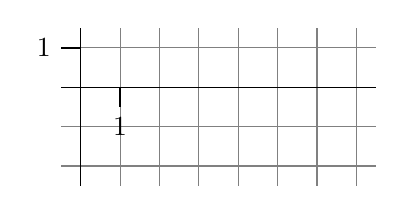
\begin{tikzpicture}[scale=0.5]
			\draw[thin,gray] (-0.5,-2.5) grid (7.5,1.5);
			\draw[\myArrow] (-0.5,0) -- (7.5,0);
			\draw[\myArrow] (0,-2.5) -- (0,1.5);
			\draw[thick] (1,0) -- ++(0,-0.5) node[below] {$1$};
			\draw[thick] (0,1) -- ++(-0.5,0) node[left] {$1$};

			\node at (2,-2) {$×$};
			\node at (4,-1) {$×$};
			\node at (6,0) {$×$};
		\end{tikzpicture}
	\end{center}
\end{frame}

\begin{frame}
	\uline{Correction Sujet de droite (B) :}

	{\color{blue}1.}

	\begin{multicols}{2}
		{\color{blue}a.} L'image de $1$ est $2$.

		L'image de $3$ est $-1$.

		L'image de $-1$ est $0$.

			{\color{blue}b.} Les antécédents de $2$ sont -$3$ et $1$.

		Les antécédents de $-1$ sont $2$ et $3$.

		L'antécédent de $2,5$ est $-3,5$.
	\end{multicols}

	{\color{blue}2.}

	\begin{multicols}{2}
		{\color{blue}a.} L'image de $3$ est $3$.

		L'image de $6$ est $9$.

		L'image de $-1$ est $-5$.

			{\color{blue}b.} L'antécédent de $-1$ est $1$.

		L'antécédent de $-9$ est $-3$.

		L'antécédent de $7$ est $5$.
	\end{multicols}

	{\color{blue}3.} On a $g(1) = -1$, $g(2) = 1$ et $g(3) = 3$ :
	\begin{center}
		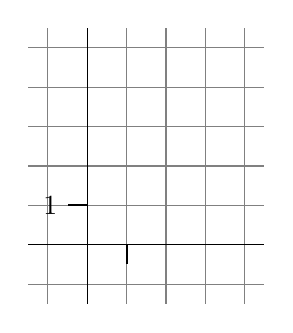
\begin{tikzpicture}[scale=0.5]
			\draw[thin,gray] (-1.5,-1.5) grid (4.5,5.5);
			\draw[\myArrow] (-1.5,0) -- (4.5,0);
			\draw[\myArrow] (0,-1.5) -- (0,5.5);
			\draw[thick] (1,0) -- ++(0,-0.5);
			\draw[thick] (0,1) -- ++(-0.5,0) node[left] {$1$};

			\node at (1,-1) {$×$};
			\node at (2,1) {$×$};
			\node at (3,3) {$×$};
		\end{tikzpicture}
	\end{center}
\end{frame}

\end{document}